\subsubsection{User Interface Mockups}
Below is the page that the user would see after logging in. 
It displays basic information about the user and previews some relevant posts.
The header that leads to various parts of the website is persistent throughout all pages.

\begin{figure}[h]
\centering % centre is you want
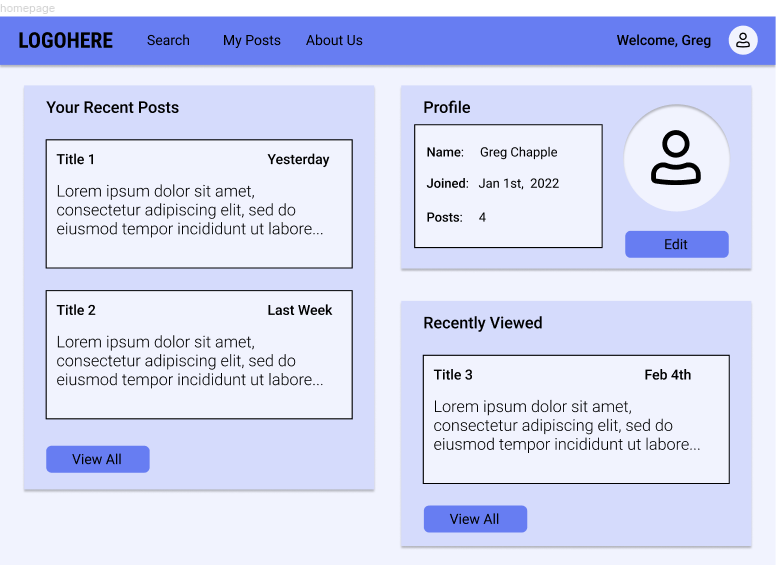
\includegraphics[scale=0.50]{homepage} % To learn more go to: https://www.overleaf.com/learn/latex/Inserting_Images 
\caption{Homepage of site mockup}
\label{fig: homepage} % Can be used with function \ref{fig: passion-fruit-flower} to reference to image
\end{figure}
\newpage

\noindent	
Here the user is shown searching for posts by a certain user. 
The page displays all posts published by that user with their title, 
data and current version.

\begin{figure}[h]
\centering % centre is you want
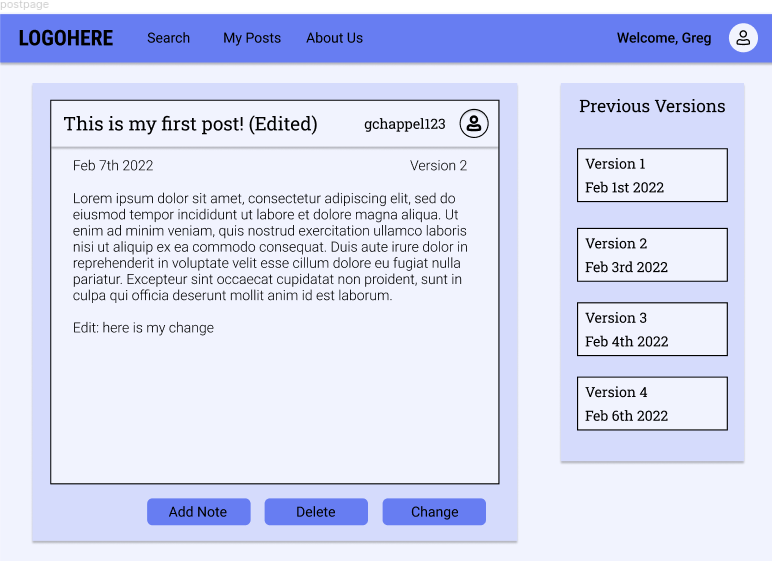
\includegraphics[scale=0.50]{postpage} % To learn more go to: https://www.overleaf.com/learn/latex/Inserting_Images 
\caption{Postpage of site mockup}
\label{fig: postpage} % Can be used with function \ref{fig: passion-fruit-flower} to reference to image
\end{figure}
\newpage

\noindent	
When clicking on a post from the search or the user's own list of posts, 
it takes the user to a page showing the entire post in its most recent version. The buttons on the right change the version of the post currently displayed.

\begin{figure}[h]
\centering % centre is you want
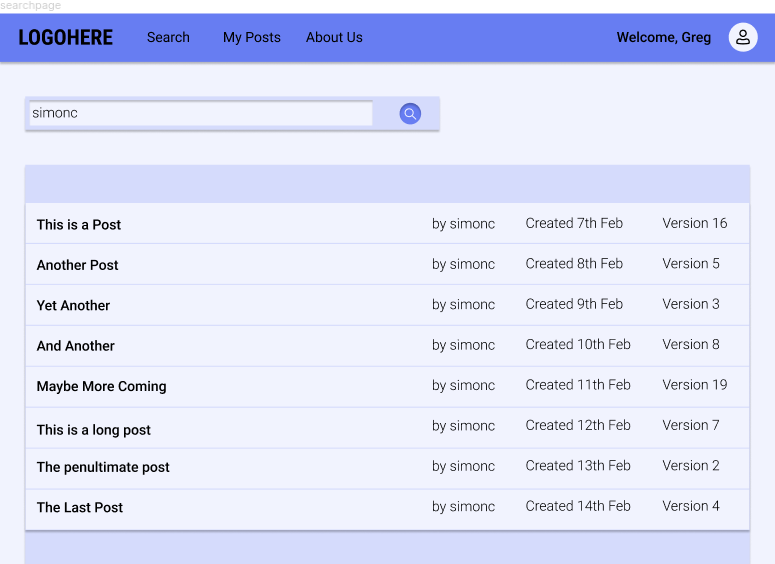
\includegraphics[scale=0.50]{searchpage} % To learn more go to: https://www.overleaf.com/learn/latex/Inserting_Images 
\caption{Seachpage of site mockup}
\label{fig: searchpage} % Can be used with function \ref{fig: passion-fruit-flower} to reference to image
\end{figure}
\newpage

\noindent
Below this is a list of the changes made to the post, 
the date the change was made and a short note explaining the change made.

\begin{figure}[h]
\centering % centre is you want
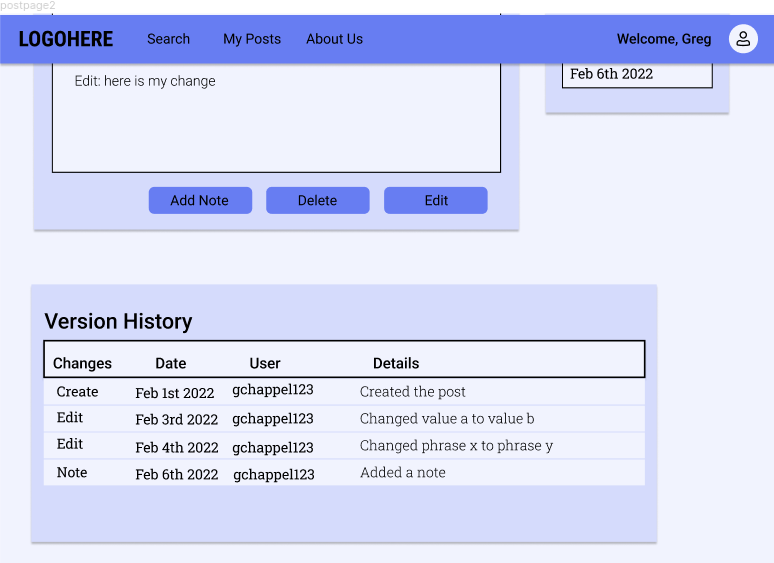
\includegraphics[scale=0.50]{postpage2} % To learn more go to: https://www.overleaf.com/learn/latex/Inserting_Images 
\caption{Postpage 2 of site mockup}
\label{fig: postepage2} % Can be used with function \ref{fig: passion-fruit-flower} to reference to image
\end{figure}
\newpage
